\chapter{LHCb software performance profiling}
\chaptermark{Performance profiling}
\section{Introduction}

In \lhcb, as in all High Energy Physics (HEP) experiments, complex software is
used to process the data recorded by the detectors. Performance is an essential
characteristic of this software, especially when dealing with HLT: its role is
to filter events coming from the hardware based trigger in order to identify
those with interesting physics, and to write them to disk in real-time. The
number of events processed per second (event rate) is therefore one of the
crucial characteristics of the HLT, as it has to keep up with the data rate
delivered by the hardware triggers ($10^6$ events per second) in order to avoid
data loss. To reach such high throughput, the processing is performed on many
nodes in parallel by highly optimized algorithms. In order to optimize the
algorithms, and to keep track of the evolution of the event rate when changes
are applied to the HLT, it is necessary to measure the overall performance of
the code but also to understand which algorithms are costly in term of Central
Processing Unit (CPU) and computer memory.

In this chapter our focus is on the analysis of frequency and duration of
function calls in algorithms (this type of analysis is commonly named CPU
profiling). Profiling helps to identify parts of the code that take a long time
to execute. In performance analysis, those places often are referenced as
hotspots. Obviously,  hotspots affect the event rate of event processing
software. So, one of the main goals of profiling HEP software is to point out
to application developers the places in the code that need to be tuned to
increase the event rate.

The first study on CPU profiling at \lhcb was carried out by Daniele Francesco
Kruse and Karol Kruzelecki in their work ``Modular Software Performance
Monitoring''~\cite{modular}. They conclude that instead of profiling the
application as a whole it would be better to divide it into modules and profile
those modules separately. In general terms, a module can be defined as an
application’s structural component that is used to group logically related
functions.  Grouping performance results by module allows a better insight into
where the performance issues are coming from. Since each module is under the
responsibility of a specific developer, the provided reports can be delivered
to the right person. For example, in the \gaudi~\cite{Barrand:2001ny} core
framework at LHCb each algorithm used for event processing is such a module
which can be profiled independently. More details on \gaudi will be given in
Section~\ref{sec:gaudi}.

This design principle was first implemented in a set of profiling tools based
on perfmon2~\cite{perfmon2} library. These tools have several drawbacks. First,
the produced analysis reports  used the  hardware event counters metrics. Only
developers with a good knowledge of the hardware  architecture could read and
interpret those reports. Since the major part of developers in HEP are
physicists, the number of users of those tools are very low. Second, since the
current tools do not use the counters multiplexing feature of perfmon2 library,
the target program should be run several times to collect all required hardware
counters. As a result, the profiling time is significantly increasing.

To fill some of the the gaps of the previous tools the Gaudi Intel
Profiling Auditor was created. This profiling tool uses the same module principle that was
described in~\cite{modular}, but is based on \iamp~\cite{vtune}.
\amp is the newer performance profiling tool, that provides better
functionality than perfmon2 library.

In the next section \iamp is briefly reviewed. Then is discussed how the Gaudi
Intel Profiling Auditor can integrate \amp to the \gaudi framework and shown
examples of using those tools to profile \lhcb's HLT.

\section[VTune Amplifier]{\iamp}
This section gives an overview of \iamp profiling tool and
describes its basic features and analysis reports.

\subsection{Overview}
\iamp is a commercial application for software performance analysis that is
available for both Linux and Windows operating systems. \amp belongs to the
runtime instrumentation class of profiling tools. This means that the code is
instrumented before execution and the program is fully supervised by the tool.
A target application can be profiled without any modification of the codebase.

\iamp has  various kinds of code analysis including hotspot analysis,
concurrency analysis, locks and waits analysis. In Profiling Auditor a
hotspot analysis based on the user-mode sampling feature of \amp i used.
User-mode sampling allows to profile a program by exploring a call stack of a
running program and produce one simple metric --- amount of time spent in the
function.

The amount of time spent in a function (CPU time) is calculated by interrupting
a process and collecting samples of call stacks from all active threads. CPU
time value is calculated by counting the number of  a function's appearances at
the top of a call stack. This means that stack sampling is a statistical method
and does not provide a 100\% accurate measurement. However, for a large number
of samples the sampling error does not have a serious impact on the accuracy of
analysis. More details about sampling accuracy will be provided in section 2.2.

\amp also supports the hardware event-based sampling and provides advanced
metrics based on event counters inside a processor. Reports that use those
metrics require  knowledge of hardware architecture  unlike the user-mode
sampling reports that can be understood by any application developers.
Furthermore, while the user-mode sampling can be performed on any 32 and 64-bit
x86 based machine, the hardware event-based sampling is targeted only for a
specific \intel microarchitecture and requires a special driver to be installed
on the operating system. The advantage of the hardware event-based sampling
that it can be used for fine tuning of algorithms in places where  the user-
mode sampling could not point out the reasons for the hotspot.

The goal of our profiling tool is to provide analysis reports to a wider
audience of software developers and, therefore, for implementation we chose the
user-mode sampling method over hardware-mode sampling.

\subsection{Sampling interval}

The sampling interval is an important parameter of the user-mode sampling
method. It can impact on results accuracy and on total profiling time. \intel
recommends to use a 10 ms interval. Using this value the average overhead of
the sampling is about 5\% in the most applications. The minimum sampling
interval value depends on the operating system. For example, a 10 ms interval
is the minimum value for the old Linux kernel 2.4, whereas 1 ms is the minimum
value for the modern Linux $\ge$ 2.6 kernels.

To determine an appropriate sampling interval, consider the duration of the
collection, the speed of your processors, and the amount of software activity.
For example, if the duration of sampling time is more than 10 minutes, consider
increasing the sampling interval to 50 milliseconds. This reduces the number of
interrupts and the number of samples collected and written to disk. The smaller
the sampling interval, the larger the number of samples.

\subsection{Tools}

\amp has two major interfaces --- a command-line tool {\it amplxe-cl} and a
Graphical User Interface tool {\it amplxe-gui}. {\it Amplxe-gui} generally
plays a role of analysis results presenter, but can also be used as a wrapper
to the  command-line tool. {\it Amplxe-cl} is used to execute the profiling
supervisor with appropriate parameters.  The second important function of {\it
amplxe-cl} is to export CPU usage reports to CSV text format. This feature
allows to use collected data not only inside \amp, but also in external user
applications.

\subsection{Profiling reports}

In this section we review essential profiling reports that are available in
\amp. These reports can be obtained either from {\it amplxe-gui} or {\it
amplxe-cl tool}, but for short we present only GUI screenshots.

An ordered function’s CPU time usage report is a basic report of almost at all
performance profilers (Figure~\ref{fig01}).

\begin{figure}[H]
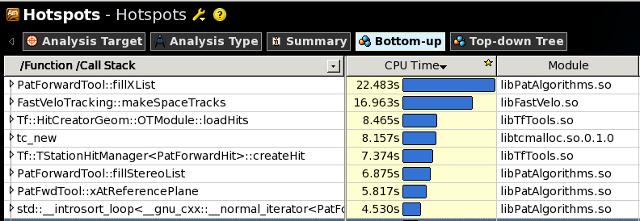
\includegraphics[width=\textwidth]{profiler/fig01.png}
\caption{Function’s CPU Time report. The first column contains
function names. The second column is a CPU time usage and the last column
contains the names of the shared libraries where the functions are defined.}
\label{fig01}
\end{figure}

\amp provides many grouping options: 
\begin{figure}[H]
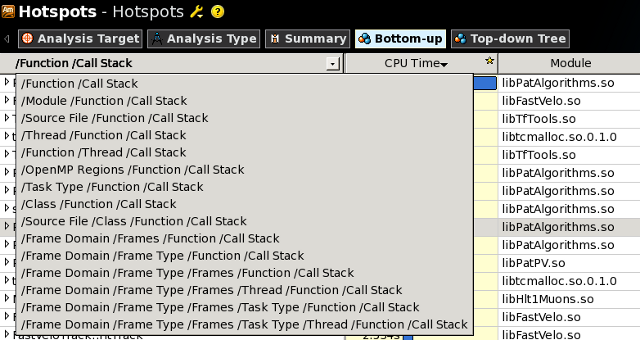
\includegraphics[width=\textwidth]{profiler/fig02.png}
\caption{Various grouping options.}
\label{fig02}
\end{figure}

Example of grouping by shared library:

\begin{figure}[H]
\begin{minipage}{\textwidth}
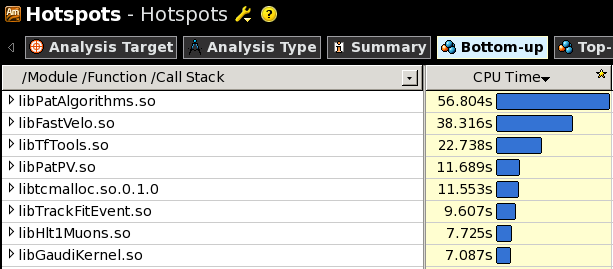
\includegraphics[width=\textwidth]{profiler/fig03.png}
\caption{\label{fig03}Shared libraries  CPU time report. First column contains
a name of shared library.}
\end{minipage}
\end{figure}


The striking feature of \amp is an ability to filter data based on a selection
in the timeline. This feature does not exists in other popular profilers:

\begin{figure}[H]
\begin{minipage}{\textwidth}
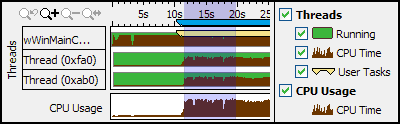
\includegraphics[]{profiler/fig04.png}
\caption{\label{fig04}Filter data on a selection in timeline.}
\end{minipage}
\end{figure}

CPU usage by code line can be created if a target application was compiled with
debug symbols:

\begin{figure}[H]
\begin{minipage}{\textwidth}
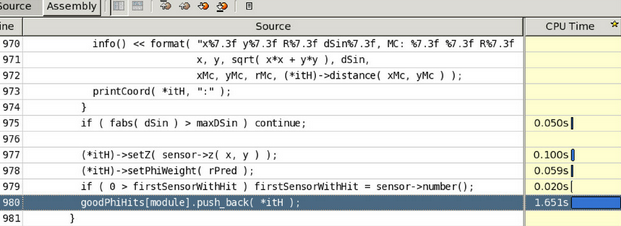
\includegraphics[width=\textwidth]{profiler/fig05.png}
\caption{\label{fig05}CPU time usage by code source line.}
\end{minipage}
\end{figure}

\subsection{Detecting code dependency}

Besides finding hotspots, another useful function of the profiling tool is to
reveal the code dependencies. Usually HEP applications have a lot of lines of
code and were developed by many people during a long period of time. Therefore,
determining relations between parts of code is very difficult. Since \amp  has
a top-down tree report of functions calls (Figure~\ref{fig06}.), we can
determine the code dependency in the application and see CPU usage in the call
chain.

\begin{figure}[H]
\begin{minipage}{\textwidth}
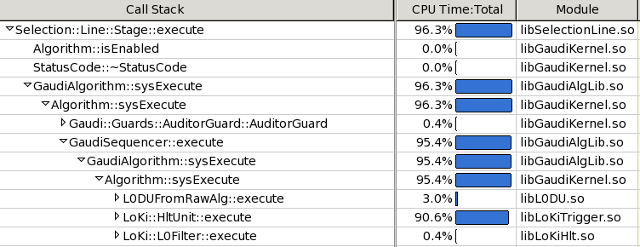
\includegraphics[width=\textwidth]{profiler/fig06.png}
\caption{\label{fig06}Top-down tree report.}
\end{minipage}
\end{figure}

\section[Profiling Auditor]{Gaudi Intel Profiling Auditor}

In the previous section we show that \iamp is a powerful performance profiling
tool. In this section is shown how this tool is used at \lhcb
for software optimization.

First, the \gaudi framework is described and then is shown how the \gaudi Intel
Profiling Auditor can enhance \amp reports.

\subsection{Gaudi}
\label{sec:gaudi}
\gaudi is a C++ software framework used to build event data processing
applications using a set of standard components. \gaudi is a core framework used
by several HEP experiments, in particular \lhcb and \atlas at \lhc. All of the
event processing applications, including simulation, reconstruction, high-level
trigger and analysis are based on this framework. By design, the framework
decouples the objects  describing the data and those implementing the
algorithms. Due to this design,  developers can concentrate only on  physics
related tasks in algorithms and usually do not care about other parts of the
framework.

\begin{figure}[H]
\begin{minipage}{\textwidth}
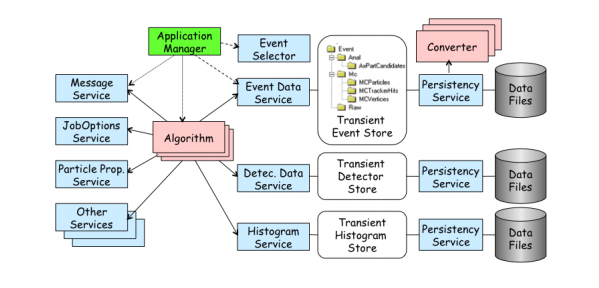
\includegraphics[width=\textwidth]{profiler/fig07.png}
\caption{\label{fig07}Gaudi Architecture (as described in
~\cite{Barrand:2001ny}). Applications are made by composing sequences of
Algorithms and adding specific Services and Tools.}
\end{minipage}
\end{figure}

The \gaudi framework is a highly customizable framework. Any component of the
system can be configured by user options.

\subsubsection{Gaudi Auditors}

The Application Manager is one of the major components of \gaudi. It takes care
of instantiating and calling algorithms. A supplement to this component  is the
Auditor Service that enable to add auditors to a \gaudi application. The auditor
is a set of user functions that are called on some workflow events in the
Manager. For example, we could add custom action that is called when the
Manager wants to execute some algorithm or when an algorithm is finished. There
are many different events types and we can add as many auditors as needed. In
other frameworks and programming languages, this type of functions are often
referenced as callback functions.

In the following section we show how we can use an auditor to build a profiling
tool.

\subsection{Profiling Auditor}

\subsubsection{Objectives.}

A \gaudi application can be profiled by \amp  without any modifications of the
codebase.  This tool can collect any data about CPU consumption in code lines,
functions, classes, shared libraries, threads, but it has one disadvantage.
\amp knows nothing about \gaudi framework's algorithms. However, algorithms are
the central point of any framework application, all major event processing
occurs there. In principle, a general task of framework users is just to write
algorithms that solve a problem and usually nothing more. So, if the profiler
could generate a report that can group function’s CPU usage by algorithm then
application developers could look to the profiling result from a new point of
view. This point of view can help to reveal previously invisible hotspots. In
order to provide such report the Gaudi Intel Profiler Auditor was developed.

\subsubsection{User API of \iamp.}

Each \gaudi algorithm has a name that is assigned to an algorithm at run-time.
\amp, in turn, is supplied with a C library that allows to import those names
to the target report. In order to use the library from user applications, the
public User API is provided in \amp. The API enables to control the data
collection process and set marks during the execution of the code. The
possibility to mark code regions at runtime is the striking feature of our new
profiling tool, because a CPU usage in the region between algorithm’s start and
finish points is what we need for the report that group functions by algorithm.
Event API is a part of the User API  that is in charge of marking.

\begin{description}
\item[\_itt\_event \_\_itt\_event\_create(const \_\_itt\_char \*name, int namelen );] \hfill \\
Create a user event type with the specified name. This API returns a handle to the user event type that should be 
passed into the following APIs as a parameter. The namelen parameter refers to the number of characters, 
not the number of bytes.

\item[int \_\_itt\_event\_start( \_\_itt\_event event );] \hfill \\
Call this API with an already created user event handle to register an instance of that event. This event appears 
in the Timeline panel display as a tick mark.

\item[int \_\_itt\_event\_end( \_\_itt\_event event );] \hfill \\
Call this API following a call to \_\_itt\_event\_start() to show the user event as a tick mark with a duration line 
from start to end. If this API is not called, the user event appears in the Timeline pane as a single tick mark.
\end{description}

\subsubsection{Implementation}

An auditor is a good component for implementing the required profiling tool. In
this case, we do not need to modify the algorithm’s code and need only to write
two callback functions: at algorithm start and finish. In order to generate the
target report those functions need to call Event API functions of \amp.

An appropriate auditor was created and named \gaudi Intel Profiling Auditor. It
was deployed to the GaudiProfiling package of \gaudi framework as a shared
library. Below we show how this profiling tool marks regions and what reports
can be generated.

\gaudi has a special type of algorithms --- Sequence. Each instance of Sequence
can execute other algorithms or sequences. So, an application's event loop
could have not only a flat but also a tree structure. Moreover, the same
algorithm instance can occur in different sequences. Therefore, it was decided
that an algorithm's region between its start and finish should be marked by the
branch identifier. In this case, we get more detailed information about usage
of the algorithm in the application. A branch identifier is constructed from an
algorithm name and its parents in the sequence tree. For example, let's profile
an application that has the following sequence tree:
\begin{verbatim}
Hlt 
    HltDecisionSequence 
        Hlt1 
            Hlt1DiMuonHighMass
                Hlt1DiMuonHighMassFilterSequence
                    Hlt1DiMuonHighMassStreamer
                        FastVeloHlt
                        MuonRec
                        Velo2CandidatesDiMuonHighMass
                    GECLooseUnit
                        createITLiteClusters
                        createVeloLiteClusters
                Hlt1DiMuonHighMassL0DUFilterSequence
                    L0DUFromRaw
                    Hlt1DiMuonHighMassL0DUFilter
\end{verbatim}

In \amp the report that use information on marked regions can be obtained by
choosing the ``Task Type / Function / Call Stack'' grouping options as seen on
Figure~\ref{fig08}.

\begin{figure}[H]
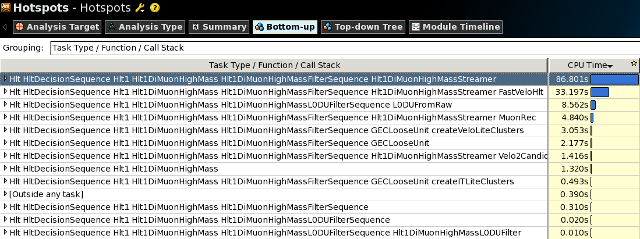
\includegraphics[width=\textwidth]{profiler/fig08.png}
\caption{Group and order CPU usage by branch identifier.}
\label{fig08}
\end{figure}

For example, the selected branch identifier {\it ``Hlt HltDecisionSequence Hlt1 Hlt1DiMuonHighMass Hlt1DiMuonHighMassFilterSequence Hlt1DiMuonHighMassStreamer''} in the report on Figure~\ref{fig08} is constructed from the names of algorithms that were executing 
when the \amp supervisor sampled a call stack. Each algorithm name in the branch is separated by the space. 

For each branch we could see a CPU usage by function (Figure~\ref{fig09}):

\begin{figure}[H]
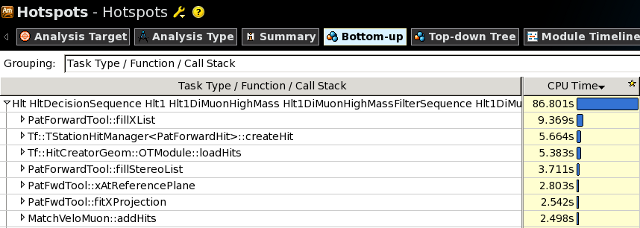
\includegraphics[width=\textwidth]{profiler/fig09.png}
\caption{Group and order CPU usage by branch identifier.}
\label{fig09}
\end{figure}

On Figure~\ref{fig09} we see the functions's CPU usage  in the algorithm {\it
Hlt1DiMuonHighMassStreamer\/} in the branch {\it ``Hlt~HltDecisionSequence~Hlt1
~Hlt1DiMuonHighMass~Hlt1DiMuonHighMassFilterSequence''}. As can be observed the
main goal was achieved --- we get the report that groups function CPU usage by
algorithm. So, the next step is only to interpret profiling results by
application developers and, if needed, to tune algorithms.

In addition to reports on algorithms, in the \gaudi Intel Profiling Auditor were
added options that allow to skip unimportant regions of the code during
profiling. Information about functions in those regions is not collected and,
as a result, we get clearer reports and a decrease of total profiling time. For
example, usually time critical processes happens in the event loop. Thus,
initialization and finalization phases are not interesting for developers. Due
to this, the auditor has options that trigger the start of  profiling on the
first event in the event loop and stop it after the last event.


\section{HLT Profiling Examples}

In the previous section we demonstrated how \gaudi Intel Profiler Auditor can
assist  in profiling \gaudi applications. The original motivation for creating
this auditor was a profiling of HLT applications of the \lhcb experiment. As was
stated in the introduction, trigger programs are most sensitive to the event
processing time. Therefore, a performance profiling is an essential tool in the
hands of trigger's applications developers. In this section we show three
examples of using \amp and \gaudi Intel Profiling Auditor to profile the \moore
application --- a \gaudi based HLT framework at \lhcb.

\subsection{Memory Allocation Functions}

In the first example we profile a \moore program twice. The first time a program
was executed with the standard memory allocation function {\it operator new\/}
from {\it libstdc++\/} library:

\begin{figure}[H]
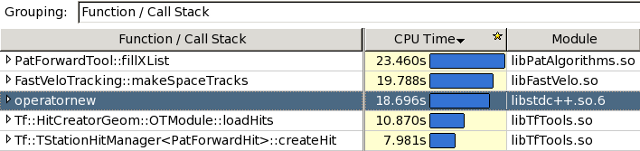
\includegraphics[width=\textwidth]{profiler/fig10.png}
\caption{Hotspot functions in the \moore application with the
standard memory allocation function.}
\label{fig10}
\end{figure}

\noindent and the second time it was executed with the memory allocation function {\it
tc\_new} from tcmalloc library~\cite{perftools}:

\begin{figure}[H]
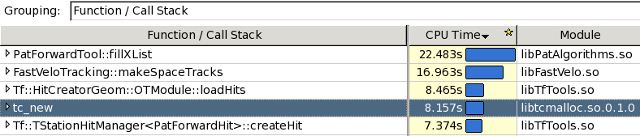
\includegraphics[width=\textwidth]{profiler/fig11.png}
\caption{Hotspot function in the \moore application with the memory allocation functions from tcmalloc 
library.}
\label{fig11}
\end{figure}

The figures indicates that {\it tc\_new} function is twice faster than {\it
operatornew}. Moreover, the total application time reduction by 5\% was
observed if we replace standard allocation functions with function from
tcmalloc library.

\subsection{Measuring Profiling Accuracy}

To check the CPU time measurement accuracy we compared the results obtained by
the \gaudi Intel Profiler Auditor and by the \gaudi Timer Auditor. The Timer
Auditor proceed  in the same way as the Profiler Auditor --- it calculates the
difference between the algorithm’s finish time and the time at the start of the
algorithm. Unlike the \gaudi Intel Profiler Auditor, the Timer Auditor
calculates the exact time spent in the algorithm. So, we can assume a CPU time
observed by the Timer Auditor as a reference value. The limitation of the Timer
is that it creates reports only for algorithms times  and could not provide
results for a low level of granularity (for functions or code instructions).
Therefore, only the algorithm’s CPU times were compared.

Since the VTune Amplifier XE instruments the code before execution, the
absolute CPU time measured by the Profiler can differ from the time measured by
the Timer auditor.  But the time distribution of all algorithms should stay the
same in both auditors.  So, for the test we took a real HLT application and run
it twice. The first time we used the Timer auditor and the second time the
\gaudi Timer Auditor was used. Then we selected five hotspot algorithms and
calculated their time distribution relative to the top hotspot algorithm. The
process was repeated three times with different numbers of events: 10
(Table~\ref{tab:tevents10}), 100 (Table~\ref{tab:tevents100}) and 1000 events
(Table~\ref{tab:tevents1000}):

\begin{table}[H]
\caption{10 events}
\label{tab:tevents10}
\begin{center}
\begin{tabular}{rrrr}\toprule
Algorithm name & Timer (\%) & Profiler (\%) & \bf{Difference} \\
\midrule
L0Muon & 100 & 100 & -\\
Hlt1TrackAllL0Unit & 63.71 & 63.571 & \bf{0.139}\\
FastVeloHlt & 33.065 & 7.143 & \bf{25.922}\\
L0Calo & 8.065 & 0 & \bf{8.065}\\
HltPVsPV3D & 4.032 & 0 & \bf{4.032}\\
\bottomrule
\end{tabular}
\end{center}
\end{table}

\begin{table}[H]
\caption{100 events}
\label{tab:tevents100}
\begin{center}
\begin{tabular}{rrrr}\toprule
Algorithm name & Timer (\%) & Profiler (\%) & \bf{Difference} \\
\midrule
L0Muon & 100 & 100 & --- \\
Hlt1TrackAllL0Unit & 36.985 & 42.353 & \bf{-5.368}\\
FastVeloHlt & 29.648 & 28.235 & \bf{1.413}\\
L0Calo & 7.94 & 15.294 & \bf{-7.354}\\
HltPVsPV3D & 2.613 & 4 & \bf{-1.387}\\
\bottomrule
\end{tabular}
\end{center}
\end{table}

\begin{table}[H]
\caption{1000 events}
\label{tab:tevents1000}
\begin{center}
\begin{tabular}{rrrr}\toprule
Algorithm name & Timer (\%) & Profiler (\%) & \bf{Difference} \\
\midrule
L0Muon & 100 & 100 & -\\
Hlt1TrackAllL0Unit & 35.872 & 35.147 & \bf{0.725}\\
FastVeloHlt & 29.648 & 28.235 & \bf{1.413}\\
L0Calo & 30.478 & 29.736 & \bf{0.742}\\
HltPVsPV3D & 2.491 & 2.25 & \bf{0.241}\\
\bottomrule
\end{tabular}
\end{center}
\end{table}

As expected, our test shows that the hotspot algorithms are the same in both
auditors and the accuracy of the CPU time distribution measured by the Profiler
is increasing while increasing the number of events. As a result, we can be
confident that the Profiler can identify the hotspots with the high precision.

\subsection{Custom reports}

In the second example is demonstrated how custom reports can be created. Basic
profiling reports can be picked up in
\amp, but if a custom report is required then a user tool needs to be created .
This application can get the CPU usage data from VTune™ Amplifier XE by using
its export function. For example, if we export CPU Time data that is shown on
Figure~\ref{fig08} then the following pie chart report can be created.

\begin{figure}[H]
\begin{minipage}{\textwidth}
\begin{center}
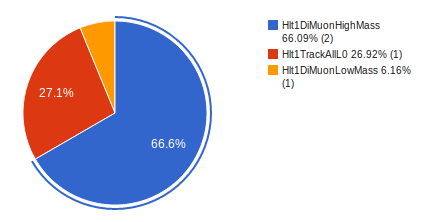
\includegraphics[width=100mm]{profiler/fig12.png}
\caption{\label{fig12}CPU Time percentage of top-level algorithms in the \gaudi sequence tree.}
\end{center}
\end{minipage}
\end{figure}

The report on Figure~\ref{fig12} was produced by a user application that took
an exported  comma-separated-values (CSV) data and compiled it to javascript
code that can be inserted to any dynamic web page.

\section{Conclusions}
In this chapter we presented the \gaudi Intel Performance Auditor --- a CPU
profiling tool that is used in \lhcb experiment at CERN. This tool integrates
the functionality of \iamp performance profiler to the \lhcb core framework
\gaudi. The key advantage of the auditor is an ability to produce reports that
use the framework's modules to present performance analysis results. Those
reports help  developers to identify hotspots in the code and improve the
application performance. Besides the reports, the \gaudi Intel Performance
Auditor provides the options that allow to control the \iamp supervisor’s
process from the \gaudi applications.

The results have further strengthened our confidence in the profiling sampling
technique. This technique gives us a reasonable overhead of total profiling
time (5\% at \iamp) in comparison to the tools that count the functions calls.
For example, the popular profiling tool Valgrind~\cite{valgrind} counts every
code instruction and programs running under this tool usually run from five to
twenty times  slower than running outside Valgrind. Though Valgrind provides
precise measurements, using the sampling technique we can get accurate results
by tuning the sampling interval or increasing the number of processing events.

Software optimization has received much attention in the last two years at
\lhcb. To obtain precise information of the general performance, to make
profiling results comparable and to verify the influences of improvements in
the framework or of specific algorithms, it is important to rely on
standardized profiling and regression tests. Software metrics can be created
from the profiling results to monitor the changes in performance and to create
reports on a regular basis if modifications lead to significant
performance degradations. Therefore, for this purpose a system for systematic
profiling is developing at \lhcb, where the \gaudi Intel Profiling Auditor
is one of the main parts.
